\chapter{Analiza literaturowa zagadnienia}
\label{cha:Analiza_literaturowa_zagadnienia}
Systemy realizujące zadanie śledzenia obiektów, rozumiane jako ciągłą obserwację zmiany stanu obiektu określonego wcześniej jako obiekt zainteresowania, charakteryzują się dużą złożonością i interdyscyplinarnością. W odniesieniu do robotyki mobilnej, w literaturze pod pojęciem ,,śledzenie obiektów'' (ang. \textit{object tracking}) rozumie się:

\begin{enumerate}

	\item \label{itm:Algorytm_przetwarzania_obrazow} Funkcję algorytmu cyfrowego przetwarzania obrazów, polegającą na wyróżnieniu obiektu zainteresowania, określeniu jego charakterystycznych właściwości oraz uaktualnieniu informacji o jego położeniu na kolejnych klatkach sekwencji video %\cite{Campoy2009, Hu2015, Liem2008, Markovic2014, Mohamed2014, Olivares-Mendez2009, Sadeghi-Tehran2014, Fernandez-Caballero2010,  Zhao2013, Park2011}

	\item \label{itm:System_sterowania} Funkcję systemu sterowania robota, dokonującego rejestracji obecności obiektu zainteresowania oraz zmiany stanu robota pozwalającej na utrzymanie tego obiektu w zasięgu pokładowych sensorów, ewentualnie przy jednoczesnej realizacji określonego zadania, np. jak największym zbliżeniu się do obiektu %\cite{Bahn2011, Campoy2009, Chen2012, Deng2010, Deng2010a, Germa2010, Han2013, Hashimoto2007, Hwang2010, Kim2011, Kim2012, Lee2011, Li2007, Liem2008, Liu2014, Markovic2014, Murakami2012, Olivares-Mendez2009, Park2011, Park2010, Rui2009, Tinh2014, Yu2008}
	
\end{enumerate}

Poniżej dokonano obszerniejszej analizy tych dwóch grup zagadnień.

\todo{Opisać powiązanie poprzez Visual Servoing}

\section{Zagadnienia z dziedziny cyfrowego przetwarzania obrazów występujące w kontekście zadania śledzenia obiektów}
\label{sec:Zagadnienia_z_dziedziny_cyfrowego_przetwarzania_obrazow}

\subsection{Ekstrakcja i deskrypcja cech obrazu}
\label{subsec:Ekstrakcja_i_deskrypcja_cech_obrazu}
Pojęcie \textbf{cechy obrazu} (ang. \textit{image feature}) jest z natury nieprecyzyjne i ogólnie może oznaczać dowolną informację związaną z obrazem, która jest przydatna w ramach wykonywania określonego algorytmu \cite{Campoy2009}. Funkcjonuje ono w literaturze również w nieco konkretniejszym ujęciu i według monografii \cite{Szeliski2011} obiekty określane cechami obrazu należą do jednej z trzech podstawowych kategorii:

\begin{enumerate}
	\item Punkty charakterystyczne (ang. \textit{keypoint features}, \textit{interest points} lub \textit{corners}) i regiony charakterystyczne (ang. \textit{blobs})
	\item Kontury obiektów na obrazie (ang. \textit{edges})
	\item Proste oraz krzywe występujące na obrazie
\end{enumerate}

Porównanie przykładowych cech obrazów należących do poszczególnych kategorii przedstawione zostało na rysunku \ref{fig:Przyklady_cech}. Ekstrakcja i deskrypcja cech jest jedną z podstawowych metod analizy obrazów i znajduje zastosowanie m.in. w algorytmach rozpoznawania obiektów, śledzenia obiektów, mozaikowania czy dopasowywania obrazów w stereoskopii. Celem wykonania takiej operacji jest wydobycie z dużej ilości informacji zawartej na obrazie jej istotnej części.

\begin{figure}[!htb]
	\begin{center}
		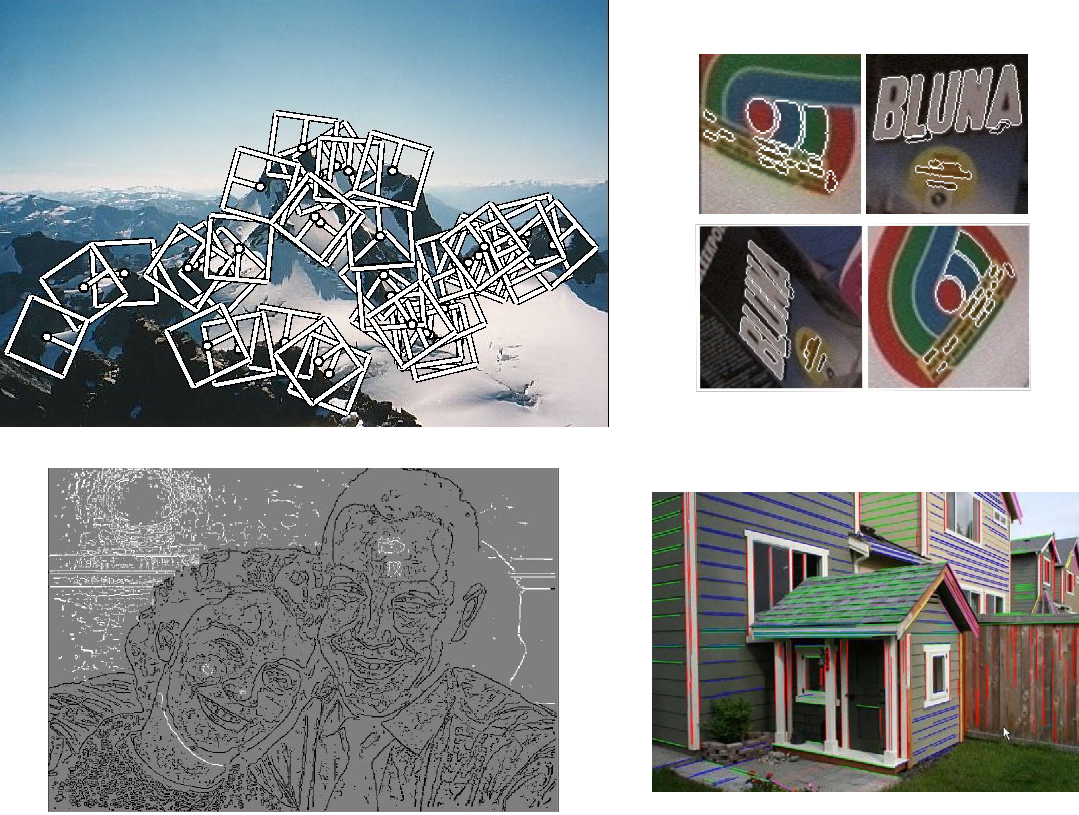
\includegraphics[width=12cm]{images/object_features.png}
	\end{center}	
	\longcaptionsource{Przykłady cech występujących na obrazach}{Od lewego górnego rogu: Punkty charakterystyczne (tutaj z wizualizacją ich przykładowych deskryptorów), regiony charakterystyczne, kontury obiektów, linie proste występujące na obrazie}{\cite{Szeliski2011}}
\label{fig:Przyklady_cech}
\end{figure}

\textbf{Punkt zainteresowania} można rozumieć jako punkt na obrazie wyróżniający się spośród otoczenia, np. narożnik występujący w konturze obiektu widocznego na obrazie. Analogicznie, \textbf{region zainteresowania} posiada cechę charakterystyczną odróżniającą go od tła, np. ma jednolity kolor. W obu przypadkach stwierdzenie ,,charakterystyczności'' odbywa się poprzez porównanie z otoczeniem. Porównanie to polega zwykle (w dużym uproszczeniu) na znalezieniu maksimów lokalnych pewnej funkcji oceniającej ,,charakterystyczność'' dla każdego punktu obrazu oraz jego lokalnego otoczenia. Po wykryciu zbioru cech wykonuje się ich \textbf{deskrypcję} (ang. \textit{feature description}), polegającą na wyznaczeniu ich formalnego opisu (zwykle w postaci wektora liczb) cechującego się zwięzłością, powtarzalnością oraz inwariantnością \cite{Szeliski2011}, tzn. odpornością na przekształcenia afiniczne, zmiany oświetlenia, szum, etc. Odbywa się to w oparciu o piksele otoczenia punktu charakterystycznego lub piksele samego regionu charakterystycznego. Granica rozróżniająca punkt charakterystyczny i region charakterystyczny jest więc bardzo niewyraźna, tym niemniej występuje w literaturze. Analizę z wykorzystaniem cech tego typu kończy ich \textbf{dopasowanie} (ang. \textit{feature matching}) lub \textbf{śledzenie} (ang. \textit{feature tracking}), np. pomiędzy dwoma kolejnymi klatkami sekwencji video lub obrazami jednej sceny zarejestrowanymi przy użyciu dwóch kamer. Model w postaci zbioru lokalnych cech, którymi są punkty charakterystyczne, nie wymaga żadnych założeń dotyczących wyglądu czy charakterystyki reprezentowanego obiektu jak całości, jak to ma miejsce np. w przypadku reprezentacji konturem. Czyni to punkty charakterystyczne odpowiednią metodą opisu obiektu w przypadku występowania zmian oświetlenia, przysłonięć i innych zakłóceń występujących powszechnie w rzeczywistych, użytkowych sekwencjach video \cite{Treiber2010}.

Ze względu na dużą użyteczność, algorytmy ekstrakcji i deskrypcji puntów charakterystycznych stanowiły w ostatniej dekadzie przedmiot intensywnych badań \cite{Treiber2010}. W literaturze zaproponowano wiele różnych podejść do tego zagadnienia, jednak jako najważniejszy przykład, dobrze obrazujący poszczególne etapy jego realizacji wymienia się algorytm \textit{SIFT} (\textit{Scale-Invariant Feature Transform}) \cite{Treiber2010} \cite{Szeliski2011}. Wykryte przy jego pomocy punkty charakterystyczne cechują się inwariantnością na zmiany skali i rotacji obrazu, a także częściowo na zmiany oświetlenia oraz zmiany widoku wynikającej z przesunięcia kamery rejestrującej scenę. Dodatkowo wykazują one dużą specyficzność (tzn. cechy odpowiadające poszczególnym fragmentom obrazu znacznie się między sobą różnią), zaś sam algorytm jest efektywny obliczeniowo \cite{Lowe2004}. Opis działania metody \textit{SIFT} zostanie poniżej przytoczony w całości.

Pierwszym krokiem algorytmu jest wyznaczenie reprezentacji obrazu w \textbf{przestrzeni skali} (ang. \textit{scale space}), w której informacja przechowywana w jego pikselach zależy nie tylko od ich współrzędnych $x$, $y$ ale również od skali $s$. Pozwala to na wykrycie punktów charakterystycznych, które pozostają stabilne przy zmianie tej skali \cite{Treiber2010}. Reprezentacja obrazu w przestrzeni skali wyznaczana jest zgodnie ze wzorem:
\begin{equation}
\label{equ:Obraz_w_przestrzeni_skali}
	L(x, y, \sigma) = G(x, y, \sigma) \ast I(x, y)
\end{equation}

\begin{equation}
\label{equ:Filtr_Gaussa}
	G(x, y, \sigma) = \dfrac{1}{\sqrt{2 \pi} \sigma ^ 2 } e^{-(x^2+y^2) / 2 \sigma^2}
\end{equation}

\noindent
gdzie:

\begin{conditions}
	x,y	& współrzędne piksela na obrazie \\
	I(x,y) & wartość piksela o współrzędnych $(x,y)$ na obrazie $I$ \\
	L(x,y,\sigma) & reprezentacja obrazu w przestrzeni skali w punkcie $(x,y)$ \\
	\sigma & rozmiar maski dla filtru Gaussa, definiujący skalę $s$ \\
	G(x,y,\sigma) & wartość maski Gaussa o rozmiarze $\sigma$ dla piksela o współrzędnych $(x,y)$\\
	\ast & operator konwolucji \\
\end{conditions}

Punkty charakterystyczne znajdują się w lokalizacjach wystąpień lokalnych minimów i maksimów reprezentacji obrazu w przestrzeni skali $L$. W celu ich wyznaczenia obliczana jest różnica obrazów w sąsiednich skalach $D(x, y, \sigma)$ \cite{Lowe2004}:
\begin{equation}
\label{equ:Roznica_obrazow}
	D(x, y, \sigma) = (G(x, y, k \sigma) - G(x, y, \sigma)) \ast I(x, y) = L(x, y, k \sigma) - L(x, y, \sigma)
\end{equation}

\noindent
gdzie:

\begin{conditions}
	k & stały współczynnik (zwykle $k \in [1,1 ; 1,4]$) \\
	D(x, y, \sigma) & Różnica filtrów Gaussa, w skrócie \textit{DoG} (z ang. \textit{Difference of Gaussian})   
\end{conditions}

Przeszukiwanie przestrzeni skali odbywa się poprzez wielokrotne wyznaczenie $D(x, y, \sigma)$, któremu towarzyszy zwiększanie $\sigma$ o stałą wartość. Lokalne ekstrema wyznaczane są poprzez porównywanie wartości $D(x, y, \sigma)$ dla współrzędnych $(x, y, \sigma)$ z punktami sąsiadującymi z punktem $(x, y)$ w skali określonej przez $\sigma$ oraz dwoma regionami o wymiarach $3 \times 3$, współśrodkowymi z $(x, y)$, o sąsiednich skalach \cite{Lowe2004}.

W ten sposób otrzymywany jest zbiór punktów charakterystycznych o określonych współrzędnych $(x, y)$ oraz skali $\sigma$. Pozycja określona tymi współrzędnymi jest jednak niedokładna - punkt charakterystyczny
może znajdować się pomiędzy pikselami (które stanowią próbki pomiarowe), dodatkowo jeden piksel w niżej skali odpowiada wielu pikselom w wyższej. Położenie ekstremów $\hat{x}$ jest wyznaczane na podstawie interpolacji funkcją kwadratową wyznaczanej poprzez rozwinięcie w szereg Taylora funkcji $G(x, y, \sigma)$ \cite{Lowe2004}:

\begin{equation}
\label{equ:Ekstrema_interpolacja}
	\hat{x} = - \frac{\partial^2 D^-1}{\partial \hat{x}^2} \frac{\partial D}{\partial \hat{x}}
\end{equation}

\noindent
gdzie:

\begin{conditions}
	\hat{x} & wektor współrzędnych w przestrzeni skali
\end{conditions}

Dodatkowo zbiór ekstremów jest filtrowany - odrzucane są niestabilne punkty charakterystyczne o niskim kontraście \cite{Lowe2004}.

\begin{equation}
\label{equ:Filtrowanie}
	D(\hat{x}) = D + \frac{1}{2} \frac{\partial D^T}{\partial \vec{x}} \hat{x}
\end{equation}

Ekstrema o wartości bezwzględnej $\abs{D(\hat{x})}$, obliczonej na podstawie równania \ref{equ:Filtrowanie}, mniejszej od wartości progowej $0.03$ są usuwane ze zbioru punktów charakterystycznych \cite{Lowe2004}.

Operacja \textit{DoG} silnie reaguje na krawędzie obecne na obrazie, co jest zjawiskiem niepożądanym, ponieważ ma charakter kierunkowy i skutkuje zdefiniowaniem niestabilnych punktów charakterystycznych
\cite{Lowe2004}. W celu ich eliminacji wprowadza się drugi etap filtracji, polegający na wyznaczeniu hesjanu $H$ (równanie \ref{equ:Hesjan}) i porównaniu jego śladu i wyznacznika z wartością progową(równanie \ref{equ:Hesjan_prog}).

\begin{equation}
\label{equ:Hesjan}
	\matr{H} = \begin{bmatrix}
		D_{xx} & D_{xy} \\
		D_{yx} & D_{yy} \\
	\end{bmatrix}
\end{equation}

\begin{equation}
\label{equ:Hesjan_prog}
	\frac{\Tr{\matr{H}}^2}{\Det{\matr{H}}} < \frac{(r + 1)^2}{r}
\end{equation}

\noindent
gdzie:
\begin{conditions}
	r & wartość progowa \\
\end{conditions}

Osiągnięcie inwariantności na obrót obrazu uzyskuje się poprzez przypisanie punktom charakterystycznym orientacji \cite{Lowe2004}. Na podstawie skali $\sigma$ punktu wyznacza się w jego środku maskę Gaussa o wariancji równej $1,5$ jego skali, w obrębie której wyznacza się moduł (równanie \ref{equ:Gradient_modul}) oraz orientację (równanie \ref{equ:Gradient_orientacja}) gradientu dla każdego piksela $(x, y)$.

\begin{equation}
\label{equ:Gradient_modul}
	m(x,y) = \sqrt{(I_s(x + 1, y) - I_s(x - 1, y))^2 + (I_s(x, y + 1) - I_s(x, y - 1))^2}
\end{equation}

\begin{equation}
\label{equ:Gradient_orientacja}
	\theta(x,y) = \arctan(\frac{I_s(x, y + 1) - I_s(x, y - 1)}{I_s(x + 1, y) - I_s(x - 1, y)})
\end{equation}

Obliczone orientacje są następnie kumulowane w histogramie z wagami określonymi poprzez odpowiadające im moduły oraz wartości okna Gaussa. Histogram składa się z $36$ przedziałów odpowiadających $360 \deg$ orientacji. Przedziały o największej liczebności odpowiadają dominującym orientacjom \cite{Lowe2004}, przy czym punktowi przypisywana jest orientacja odpowiadająca najliczniejszemu przedziałowi oraz wszystkie inne orientacje, dla których liczebności wynoszą przynajmniej $80 \%$ maksymalnej (punkt może mieć wiele orientacji jednocześnie).

\begin{figure}[!htb]
	\begin{center}
		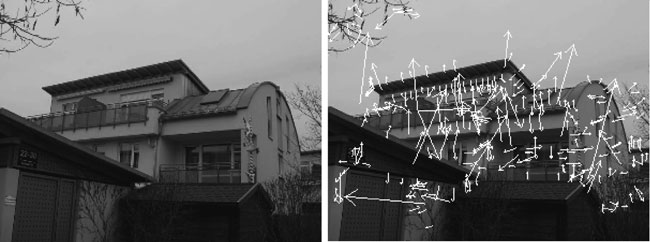
\includegraphics[width=12cm]{images/sift_extraction_description_example.png}
	\end{center}	
	\longcaptionsource{Przykład ekstrakcji i deskrypcji punktów charakterystycznych metodą \textit{SIFT}}{Punkty charakterystyczne zlokalizowane są w początkach białych strzałek, wizualizujących ich dominujące orientacje (kierunek) oraz skale (długość). Na przykładowym obrazie wykryto 289 punktów charakterystycznych.}{\cite{Treiber2010}}
\label{fig:SIFT_przyklad}
\end{figure}

Na podstawie lokalnych orientacji wyznaczany jest również deskryptor punktu charakterystycznego. Na region o wymiarach $16 \times 16$ pikseli o środku w punkcie charakterystycznym nakładana jest maska Gaussa o wariancji równej połowie jego wielkości. Następnie region ten jest dzielony na tablicę $4 \times 4$ podregionów, w obrębie których następuje akumulacja orientacji w histogramach o $8$ przedziałach (analogicznie jak w wyznaczaniu orientacji samego punktu, z wagami odpowiadającymi modułowi oraz wartości okna Gaussa) \cite{Lowe2004}. W ten sposób powstaje wektor zawierający $4 \times 4 \times 8 = 128$ elementów, opisujących punkt charakterystyczny. Końcowym etapem algorytmu jest wykonanie normalizacji, progowania ograniczającego wartość elementów do $0.2$ (próg wyznaczony eksperymentalnie) oraz renormalizacji. W ten sposób uzyskiwana jest inwariantność na zmiany iluminacji \cite{Lowe2004}. Deskryptory pozwalają na wykonanie dopasowania pomiędzy punktami charakterystycznymi (np. wykrytymi na dwóch różnych ujęciach, przedstawiających ten sam obiekt), np. przy pomocy algorytmu k-najbliższych sąsiadów (ang. \textit{k nearest neighbours}) z zastosowaniem metryki euklidesowej. Przykładowy wynik ekstrakcji i deskrypcji punktów charakterystycznych z wykorzystaniem algorytmu \textit{SIFT} przedstawiono na rysunku \ref{fig:SIFT_przyklad}.

Pomimo swoich zalet, punkty charakterystyczne nie zawsze stanowią optymalny sposób reprezentacji cech obiektu. Istnieje liczna grupa zagadnień, w których istotna jest informacja o obiekcie jako o całości, w szczególności o jego właściwościach geometrycznych. Przykładowo, są one kluczowe w zadaniu automatycznego rozpoznawania znaków drogowych lub wykrywania produktów na przenośniku taśmowym w oparciu o szablony zdefiniowane w postaci ich modeli CAD \cite{Treiber2010}. W takich przypadkach analizę obrazu przeprowadza się w oparciu o wykryte na nim \textbf{krawędzie}.

Krawędzie można zdefiniować jako granice pomiędzy regionami obrazu o różnym kolorze, intensywności bądź teksturze \cite{Szeliski2011}. Wykrywanie tych granic jest jednak zadaniem trudnym i stanowi osobną, złożoną dziedzinę cyfrowego przetwarzania obrazów noszącą nazwę segmentacji \cite{Szeliski2011}. Alternatywnie, na potrzeby zadania ekstrakcji cech, krawędzie można zdefiniować w ujęciu ,,lokalnym'' - jako wystąpienia nagłych zmian intensywności pikseli, czyli formalnie jako punkty, w których modułu lokalnego gradientu funkcji intensywności (równanie \ref{equ:Gradient_definicja}) przyjmuje duże wartości \cite{Szeliski2011}.

\begin{equation}
\label{equ:Gradient_definicja}
	\vec{J}(\vec{x}) =  \nabla I (\vec{x}) = (\frac{\partial I}{\partial x}, \frac{\partial I}{\partial y})(\vec{x})
\end{equation}

\noindent
gdzie:

\begin{conditions}
	\vec{J}(\vec{x}) & wartość gradientu funkcji intensywności dla współrzędnych $\vec{x}$ \\
	\vec{x} & wektor współrzędnych piksela $(x, y)$ \\
\end{conditions}

W praktyce obliczanie gradientu obrazu polega na wykonaniu jego splotu z odpowiednimi maskami, mającymi charakter kierunkowy. W wyniku takiej operacji otrzymuje się przybliżone pochodne kierunkowe obrazu, na podstawie których można następnie wyznaczyć moduł i orientację gradientu. Operacja wyznaczenia pochodnej obrazu wzmacnia wpływ składowych o wysokiej częstotliwości, w tym zakłóceń \cite{Szeliski2011}. Rozmiar maski oraz wagi jej elementów wpływają na zdolność filtru do uśredniania obrazu, a tym samym zmniejszania wpływu tych zakłóceń. Jednocześnie od tych parametrów zależy ogólne zniekształcenie obrazu (utrata informacji) i złożoność obliczeniowa całej operacji. W literaturze istnieje wiele propozycji masek o optymalnych właściwościach, jako przykład można podać maskę Sobela o rozmiarze $3 \times 3$ \cite{Treiber2010}. Jej postać dla kierunku poziomego $k_{S,x}$ oraz pionowego $k_{S,y}$ przedstawiono na równaniu \ref{equ:Maska_Sobela}.

\begin{equation}
\label{equ:Maska_Sobela}
	\matr{k_{S,x}} = \frac{1}{4} \begin{bmatrix} -1 & 0 & 1 \\ -2 & 0 & 2 \\ -1 & 0 & 1 \\ \end{bmatrix}
	\, \, \, \, \, \,
	\matr{k_{S,y}} = \frac{1}{4} \begin{bmatrix} 1 & 2 & 1 \\ 0 & 0 & 0 \\ -1 & -2 & -1 \\ \end{bmatrix}
\end{equation}

Po obliczeniu gradientów kierunkowych $I_x$ i $I_y$ moduł $I_G$ i orientację $I_\theta$ gradientu można wyliczyć z równania:
\begin{equation}
\label{equ:Modul_orientacja_gradientu}
	I_G = \abs{I_x} + \abs{I_y}
	\, \, \, \, \, \,
	I_\theta = \arctan \frac{I_y}{I_x}
\end{equation}

Przykład działania operatora Sobela przedstawiono na rysunku \ref{fig:Sobel_przyklad}.

\begin{figure}[!htb]
	\begin{center}
		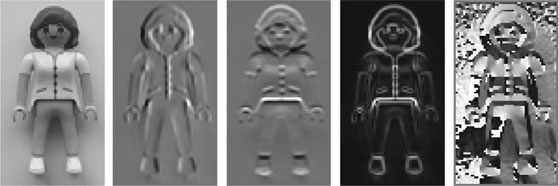
\includegraphics[width=12cm]{images/sobel_kernel_example.png}
	\end{center}	
	\longcaptionsource{Przykład wykrywania krawędzi z wykorzystaniem operatora Sobela}{Od lewej: obraz wejściowy w skali szarości; gradient poziomy (jasny kolor - wartości dodatnie, ciemny kolor - wartości ujemne); gradient pionowy (jasny kolor - wartości dodatnie, ciemny kolor - wartości ujemne); moduł gradientu; orientacja gradientu}{\cite{Treiber2010}}
\label{fig:Sobel_przyklad}
\end{figure}

Innym sposobem usuwania zakłóceń wykonanie wstępnej filtracji dolnoprzepustowej, przy czym stosowany filtr powinien być kołowo-symetryczny \cite{Szeliski2011} (powinien wygładzać obraz w każdym kierunku). Najczęściej wykorzystywany jest filtr Gaussa, posiadający tą właściwość. Ze względu na liniowość operacji różniczkowania i splotu, gradient filtrowanego obrazu można wyliczyć z równania \ref{equ:Gradient_filtrowany} \cite{Szeliski2011}.
\begin{equation}
\label{equ:Gradient_filtrowany}
	\vec{J_{\sigma}}(\vec{x}) =  \nabla (G_{\sigma}(\vec{x}) \ast I (\vec{x})) = (\nabla G_{\sigma})(\vec{x}) \ast I(\vec{x})
\end{equation}

\noindent
gdzie:

\begin{conditions}
	G_{\sigma} & maska filtru Gaussa o wariancji $\sigma$ \\
\end{conditions}

Gradient przefiltrowanego obrazu można więc wyznaczyć poprzez wykonanie jednej operacji konwolucji pomiędzy nim a poziomymi i pionowymi pochodnymi cząstkowymi maski Gaussa \cite{Szeliski2011}.

Częstym wymaganiem stawianym algorytmom wykrywania krawędzi jest ograniczenie zbioru wynikowego do krawędzi izolowanych, tj. zbioru pojedynczych pikseli zlokalizowanych wzdłuż krawędzi \cite{Szeliski2011}. W celu wyodrębniania tych pikseli należy znaleźć w całym zbiorze pikseli krawędzi elementy o maksymalnym module gradientu w kierunku prostopadłym do samej krawędzi \cite{Szeliski2011}. Realizacja tego zadania sprowadza się do wyznaczenia pochodnej kierunkowej obliczonego wcześniej gradientu wzdłuż jego kierunku (zgodnie z równaniem \ref{equ:Laplasjan_filtru_Gaussa}) oraz odnalezienia punktów zmiany jej znaku (ang. \textit{zero crossing}) \cite{Szeliski2011}.
\begin{equation}
\label{equ:Laplasjan_filtru_Gaussa}
	S_\sigma (\vec{x}) = \nabla \vec{J_{\sigma}} (\vec{x}) = \nabla^2 G_\sigma (\vec{x}) \ast I(\vec{x}
\end{equation}

\noindent
gdzie:

\begin{conditions}
	\nabla^2 & laplasjan \\
	S_\sigma (\vec{x}) & wartość funkcji znaku dla współrzędnych $\vec{x}$ \\
\end{conditions}

Maska po wykonaniu splotu $\nabla^2 G_\sigma (\vec{x})$ nazywana jest laplasjanem filtru Gaussa (ang. \textit{Laplacian of Gaussian}, w skrócie \textit{LoG}). Ze względu na złożoność obliczeniową operacja \textit{LoG} jest często aproksymowana przez przytoczoną wcześniej operacją \textit{DoG} \cite{Szeliski2011}. Wykrywanie zmiany znaku odbywa się poprzez porównanie wartości funkcji znaku $S_\sigma$ dla dwóch sąsiednich pikseli. W przypadku jej wystąpienia, na podstawie współrzędnych tych pikseli określane jest położenie punktu należącego do krawędzi (może mieć on charakter sub-pikselowy), oraz, ewentualnie interpolowana jest wartość jego gradientu \cite{Szeliski2011}. Punkt sklasyfikowany jako należący do krawędzi bywa w literaturze określany jako \textit{edgel} \cite{Szeliski2011} (połączenie słów \textit{edge} i \textit{element}).

Przedstawione wyżej metody wykrywania krawędzi operują jedynie na obrazach w skali szarości. Trywialnym sposobem rozszerzenia dziedziny ich działania na obrazy kolorowe jest osobne wykonanie dla każdej składowej koloru. Może to jednak prowadzić do wystąpienia niepożądanych zjawisk, takich jak np. wzajemne znoszenie się gradientów różnych składowych przy ich sumowaniu \cite{Szeliski2011}. Istnieją bardziej zaawansowane algorytmy rozwiązania tego problemu, nie zostaną jednak omówione w niniejszej pracy. 

Kolejnym zagadnieniem związanym z wykrywaniem krawędzi jest łączenie pikseli krawędzi izolowanych w ciągłe \textbf{kontury}, które w zależności od zastosowania, mogą być bardziej użyteczne \cite{Szeliski2011}. Kontur jest listą lub posortowaną tablicą punktów krawędzi \cite{Szeliski2011}, ma więc strukturę uporządkowaną. Jeżeli punkt krawędzi wykryto na podstawie zmiany znaku pewnej funkcji (jak, np. opisano powyżej), operacja łączenia w ciąg sprowadza się do wybrania jednego elementu i dołączaniu jego kolejnych sąsiadów w obu kierunkach \cite{Szeliski2011}.

W wyniku operacja łączenia punktów krawędzi otrzymuje się reprezentację krzywej w przestrzeni 2-D w postaci należących do niej punktów \cite{Szeliski2011}. Na ich podstawie można następnie wykonać aproksymację, mającą na celu uzyskanie reprezentacji w postaci \textbf{prostej lub krzywej opisanej równaniami matematycznymi}. Przy zastosowaniu odpowiednich metod (w szczególności transformaty Hougha) jest to możliwe nawet w przypadku wystąpienia na obrazie przerw lub przysłonięć konturu \cite{Szeliski2011}. Same cechy o tej postaci nie są jednak użyteczne w przypadku zadania śledzenia obiektów, wobec czego zagadnienie to nie zostanie szerzej omówione.

\subsection{Analiza ruchu i przepływ optyczny}
\label{subsec:Analiza_ruchu_i_przeplyw_optyczny}

Analiza ruchu obserwowanego w sekwencji obrazów jest kwintesencją algorytmów śledzenia obiektów, oraz wielu innych, jak np. kompresja video (w tym \textit{MPEG} i \textit{H.263}), stabilizacja obrazu, obrazowa diagnostyka medyczna, rekonstrukcja sceny 3-D na podstawie obrazu z poruszającej się kamery, etc. \cite{Szeliski2011}. Ze względu na postać przetwarzanych danych - sekwencje zamiast pojedynczych obrazów - analiza ruchu jest stosunkowo wymagająca obliczeniowo oraz pamięciowo. 

\begin{figure}[!htb]
	\begin{center}
		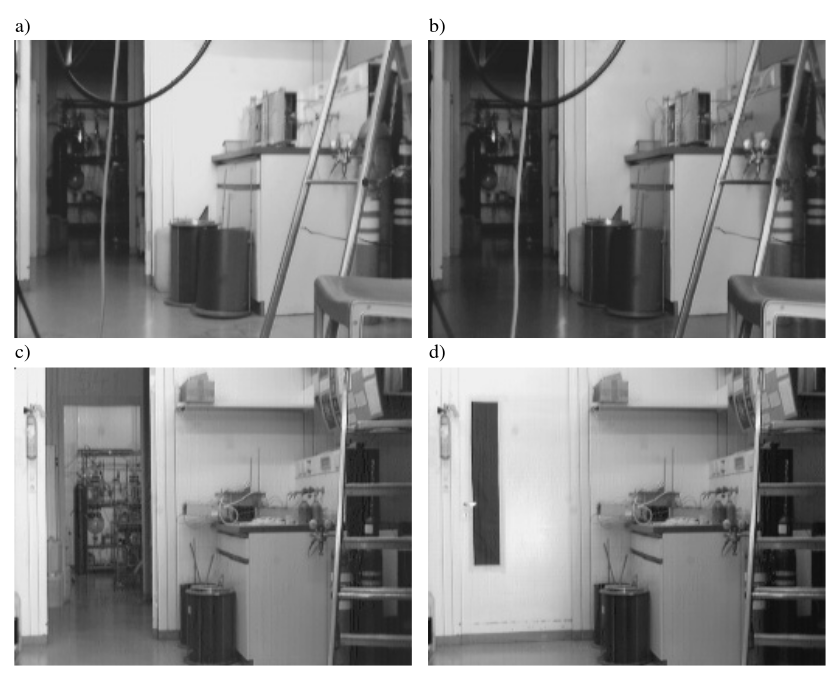
\includegraphics[width=12cm]{images/motion_illumination_change_example.png}
	\end{center}	
	\longcaptionsource{Przykład różnic pomiędzy kolejnymi obrazami sekwencji}{Definicja par: a) poprzedza b); c) poprzedza d)}{\cite{Jaehne2005}}
\label{fig:Zmiany_w_sekwencji_przyklad}
\end{figure}

Intuicyjnie, opiera się ona na obserwowaniu różnic pomiędzy dwoma kolejnymi klatkami \cite{Jaehne2005}. W trywialnym ujęciu, można ją zrealizować właśnie poprzez odjęcie od siebie dwóch kolejnych klatek, czyli poprzez wyznaczenie różnicy wartości pikseli o tych samych współrzędnych. Takie podejście okazuje się jednak bardzo szybko prowadzić do błędnej interpretacji, ponieważ zmiany wartości pikseli wynikają nie tylko z ruchu obiektów, ale również z występujących zmian iluminacji \cite{Jaehne2005}. Mogą mieć one charakter globalny - zmienia się oświetlenie całej sceny, lub lokalny - przemieszczenie lub inna zmiana stanu obiektu na scenie zmienia sposób w jaki odbija on światło, tym samym zmieniając iluminację innych obiektów w jego otoczeniu. Przykładowo, na rysunku \ref{fig:Zmiany_w_sekwencji_przyklad} przedstawiono dwie pary obrazów tej samej sceny a na rysunku \ref{fig:Roznica_obrazow_przyklad} różnice pomiędzy obrazami tych par. W pierwszej z nich zmianie ulega oświetlenie całej sceny, zmianie ulega iluminacja całej sceny, nie występuje natomiast ruch obiektów, co objawia się ogólną, niewielką zmianą wartości pikseli. W drugiej zamknięcie drzwi, a więc ich ruch, skutkuje dużą zmianą wartości pikseli przynależących do ich obszaru oraz niewielkimi lokalnymi zmianami widocznymi na innych obiektach.

\begin{figure}[!htb]
	\begin{center}
		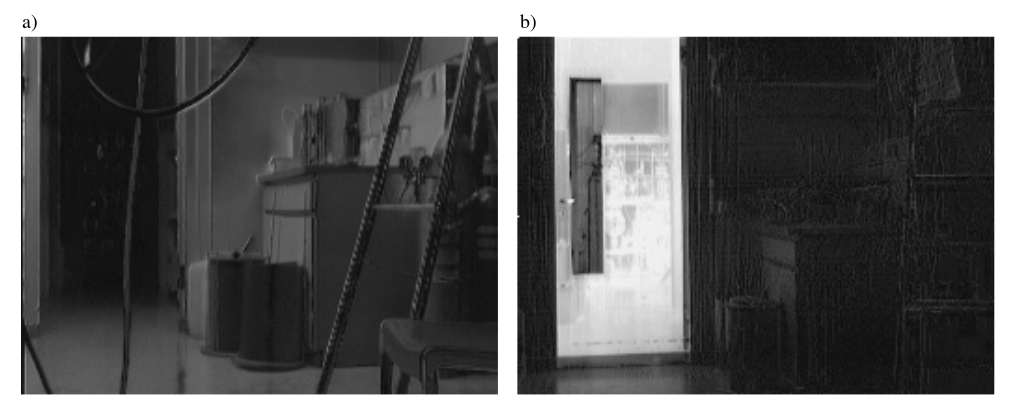
\includegraphics[width=12cm]{images/image_difference_example.png}
	\end{center}	
	\longcaptionsource{Przykład wyniku operacji odejmowania dwóch kolejnych obrazów sekwencji}{Objaśnienie: a) odejmowanie obrazów z rysunku \ref{fig:Zmiany_w_sekwencji_przyklad} a) i b); b) odejmowanie obrazów z rysunku \ref{fig:Zmiany_w_sekwencji_przyklad} c) i d)}{\cite{Jaehne2005}}
\label{fig:Roznica_obrazow_przyklad}
\end{figure}

Ruch na sekwencji obrazów ujawnia się więc poprzez zmiany wartości pikseli o charakterze przestrzennym i czasowym \cite{Jaehne2005}. W celu jego analizy konieczna jest wiedza o związku pomiędzy punktami na obrazie pierwotnym i następującym, tzn. zdefiniowanie wektorów przemieszczeń, co nie zawsze jest to możliwe w sposób jednoznaczny. Przykładowo, na obrazie obserwowany jest pewien region $x_i$ (rysunek \ref{fig:Problem_apertury}). W zależności od sposobu jego zdefiniowania, ścisłe określenie korespondencji pomiędzy tym regionem a odpowiadającym mu regionem na następnym obrazie sekwencji może być możliwe (rysunek \ref{fig:Problem_apertury}a) lub nie (rysunek \ref{fig:Problem_apertury}b i c). Zjawisko to nosi nazwę \textbf{problemu apertury}.

\begin{figure}[!htb]
	\begin{center}
		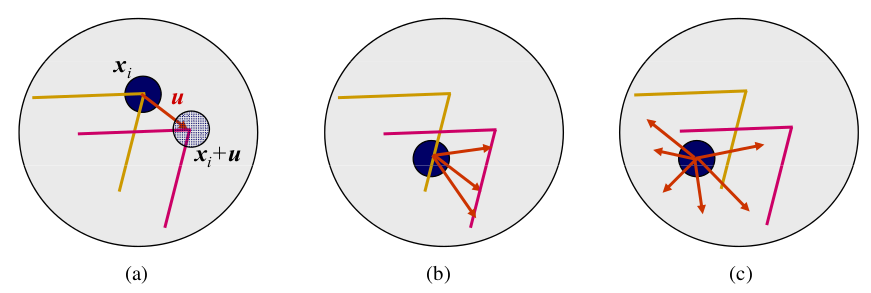
\includegraphics[width=12cm]{images/aperture_problem.png}
	\end{center}	
	\longcaptionsource{Warunki wystąpienia problemu apertury}{Krawędź obiektu zainteresowania na obrazie pierwotnym oznaczono kolorem żółtym, na obrazie następującym kolorem fioletowym. Zdefiniowano pewien region opisywany przez współrzędne jego środka $x_i$, poszukiwany jest wektor przemieszczenia $u$, pozwalający na wyznaczenie jego kolejnych współrzędnych. Możliwe przypadki: a) wektor $u$ może zostać wyznaczony w sposób jednoznaczny; b) ze względu na informacje zawarte w wybranym regionie $x_i$ na obrazie następującym można wyznaczyć wiele dopasowanych do niego regionów $x_i + u$, tzn. wektor $u$ może przyjąć wiele różnych postaci; c) informacje zawarte w regionie $x_i$ nie narzucają żadnych więzów dotyczących jego kolejnego położenia}{\cite{Szeliski2011}}
\label{fig:Problem_apertury}
\end{figure}

Problem apertury jest szczególnym przypadkiem \textbf{problemu korespondencji}, polegające na niemożliwości określenia korespondencji punktów na dwóch kolejnych obrazach w sekwencji \cite{Jaehne2005}. Jego naturę dobrze przedstawia przykład z rysunku \ref{fig:Problem_korespondencji}, na którym przedstawiono zbiór poruszających się, identycznych cząsteczek. Utworzenie powiązań pomiędzy ich pierwotnymi a wtórnymi wystąpieniami jest wykonalne, o ile odległości pomiędzy nimi są znacząco większe od długości wektorów przesunięć (rysunek \ref{fig:Problem_korespondencji}a), w przeciwnym wypadku jest niemożliwe (rysunek \ref{fig:Problem_korespondencji} b)). Zjawisko to można ograniczyć zwiększając częstotliwość próbkowania obrazów, co przekłada się na zmniejszenie modułów wektorów przesunięć \cite{Jaehne2005}. Jego całkowita eliminacja nie jest jednak możliwa przy braku założenia minimalnej dopuszczalnej odległości między cząsteczkami.

\begin{figure}[!htb]
	\begin{center}
		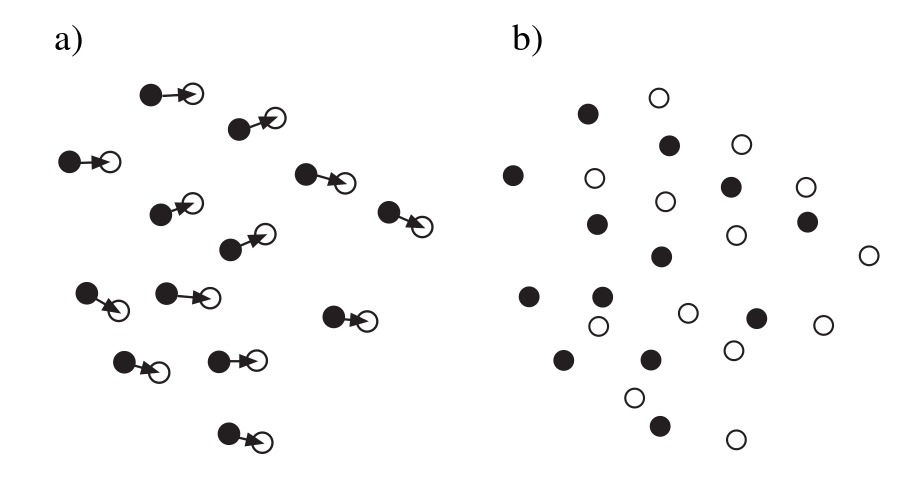
\includegraphics[width=12cm]{images/correspondence_problem.png}
	\end{center}	
	\longcaptionsource{Przykład występowania problemu korespondencji}{Czarne koła obrazują pierwotne a białe wtórne położenia nierozróżnialnych cząsteczek. Występowanie problemu korespondencji: a) względne przesunięcia cząsteczek są małe w porównaniu do odległości między nimi, dopasowanie polega na odnalezieniu najbliższej cząsteczki; b) duże wartości modułów wektorów przesunięć uniemożliwiają wykonanie dopasowania}{\cite{Jaehne2005}}
\label{fig:Problem_korespondencji}
\end{figure}

Przedstawione powyżej przykłady obrazują podstawowy problem analizy ruchu, tzn. brak identyczności pomiędzy fizyczną korespondencją rzeczywistych obiektów a wizualną korespondencją występującą na obrazie \cite{Jaehne2005}. Określenie wizualnej korespondencji pomiędzy obiektami na dwóch obrazach jest możliwe, nawet jeżeli nie występuje pomiędzy nimi fizyczna korespondencja, natomiast fizyczna korespondencja dwóch obiektów nie musi skutkować ich wizualną korespondencją na obrazie \cite{Jaehne2005}.

W celu uchwycenia zależności pomiędzy ruchem występującym w sekwencji obrazów a zmianami wartości pikseli konieczne jest wprowadzenie dwóch pojęć - \textbf{pola ruchu} (ang. \textit{motion field}) oraz \textbf{przepływu optycznego} (ang. \textit{optical flow}) \cite{Jaehne2005}. Pole ruchu $\vec{u} = [u_1, u_2]^T = [u, v]^T$ to pole wektorów rzeczywistego ruchu obiektów w przestrzeni trójwymiarowej rzutowanych na dwuwymiarową płaszczyznę obrazu, określone dla każdego jego piksela, o wymiarze prędkości \cite{Jaehne2005} \cite{Baker2011}. Przepływ optyczny $\vec{f} = [f_1, f_2]^T$ jest estymacją pola ruchu \cite{Szeliski2011}, wyznaczaną na podstawie obserwowanych przemieszczeń (,,przepływu'') poszczególnych pikseli obrazu rozróżnianych poprzez ich wartość \cite{Jaehne2005} \cite{Baker2011} \cite{Horn1981}. Pole ruchu i przepływ optyczny są identyczne tylko jeśli obiekty poruszające się na scenie nie zmieniają irradiancji płaszczyzny obrazu \cite{Jaehne2005}. Przykładową sekwencję obrazów oraz wyznaczony dla niej przepływ optyczny przedstawiono na rysunku \ref{fig:Przeplyw_optyczny}.

\begin{figure}[!htb]
	\begin{center}
		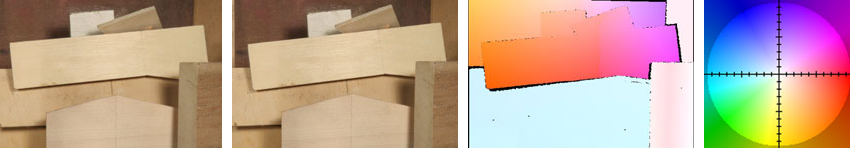
\includegraphics[width=16cm]{images/optical_flow_example.png}
	\end{center}	
	\longcaptionsource{Przykład wizualizacji przepływu optycznego}{Od lewej: dwa kolejne obrazy sekwencji, wizualizacja wyznaczonego przepływu optycznego, kodowanie wartości przepływu (jednostki na osiach mają wymiar pikseli). Pomiędzy klatkami nastąpił ruch sztywnego obiektu na pierwszym planie, tło pozostało nieruchome (brak ruchu kamery)}{\cite{Baker2011}}
\label{fig:Przeplyw_optyczny}
\end{figure}

Przepływ optyczny obliczany jest dla każdego piksela obrazu. Większość metod jego wyznaczania opiera się o optymalizację pewnej funkcji globalnej energii $E_G$ o postaci \cite{Baker2011}:
\begin{equation}
\label{equ:Energia_globalna}
	E_G = E_D + \lambda E_P
\end{equation}

\noindent
gdzie:

\begin{conditions}
	E_D & term danych - określenie stopnia spójności przepływu optycznego \\
	E_P & term nadrzędny - dookreślający problem poprzez preferowanie przepływów o określonym charakterze (np. płynnych) \\
	\lambda & współczynnik wagowy \\
\end{conditions}

Podstawowa definicja termu danych opiera się o założenie \textbf{warunku stałej jasności} (ang. \textit{brightness constancy}), tzn. że piksel odpowiadający pojedynczemu punktowi poruszającego się obiektu zmieniając położenie na obrazie nie zmienia swojej wartości lub koloru \cite{Baker2011}. Formalną postać tego warunku przedstawia równanie \ref{equ:Warunek_stalej_jasnosci}. 
\begin{equation}
\label{equ:Warunek_stalej_jasnosci}
	I(x, y, t) = I(x + u, y + v, t + 1)
\end{equation}

\noindent
gdzie:

\begin{conditions}
	I(x, y, t) & wartość piksela $(x, y)$ na obrazie $I$ w chwili $t$ \\
	(u(x, y, t), v(x, y, t)) & przepływ \\
\end{conditions}

Rozwinięcie równania \ref{equ:Warunek_stalej_jasnosci} w szereg Taylora pierwszego rzędu pozwala na wyznaczenie \textbf{równania przepływu optycznego} (ang. \textit{optical flow constraint}):
\begin{equation}
\label{equ:Rownanie_przeplywu_optycznego}
	u \frac{\partial I}{\partial x} + v \frac{\partial I}{\partial y} + \frac{\partial I}{\partial t} = 0
\end{equation}

Równania \ref{equ:Warunek_stalej_jasnosci} i \ref{equ:Rownanie_przeplywu_optycznego} zawierają po dwie niewiadome, elementy nieznanego przepływu $u(x, y, t), v(x, y, t)$, przy jednoczesnym narzuceniu pojedynczego ograniczenia. Oznacza to, że zagadnienie wyznaczenia przepływu jest niedookreślone, stąd konieczność wprowadzenia do równania \ref{equ:Energia_globalna} termu nadrzędnego. Jest to również formalna przyczyna występowania wspomnianego wcześniej problemu apertury \cite{Baker2011}. Oba równania mogą służyć do wyznaczenia postaci termu danych, przy czym ich znaczenie jest praktycznie tożsame, alternatywę stanowi założenie o wysokim współczynniku korelacji pomiędzy dwoma kolejnymi obrazami \cite{Baker2011}. Stosowane równanie jest przekształcane do postaci, z której wylicza się wartość błędu dla każdego piksela. Wartości błędów są następnie agregowane, w wyniku czego otrzymuje się funkcję kary, jak np. w algorytmie Horna-Schuncka \cite{Horn1981} \cite{Baker2011} \cite{Karasulu2013}:
\begin{equation}
\label{equ:Funkcja_kary}
	E_D = \sum\limits_{x,y} (u \frac{\partial I}{\partial x} + v \frac{\partial I}{\partial y} + \frac{\partial I}{\partial t})^2
\end{equation}

W celu zwiększenia odporności na zmiany wyglądu sceny nie wynikające z ruchu, niektóre metody zamiast wartości pikseli używają cech, np. opisanych w podrozdziale \ref{subsec:Ekstrakcja_i_deskrypcja_cech_obrazu} punktów charakterystycznych \textit{SIFT} \cite{Baker2011}, lub innych, specjalnie do tego przystosowanych. 
Zwiększenie odporności można również uzyskać poprzez wprowadzenie do równania \ref{equ:Warunek_stalej_jasnosci} zmiany wartości piksela wprost \cite{Baker2011}

\begin{equation}
\label{equ:Warunek_stalej_jasnosci_zmodyfikowany}
	g(x,y) I(x, y, t) = I(x + u, y + v, t + 1) + b(x, y)
\end{equation}

\noindent
gdzie:

\begin{conditions}
	g(x,y) & współczynnik skalujący \\
	b(x,y) & współczynnik przesunięcia \\
\end{conditions}

Oczywistą konsekwencją takiego działania jest zwiększenie liczby niewiadomych do czterech, wymaga więc ono narzucenia na zmiany zmianę wartości piksela zdefiniowaną przez $g(x,y)$ i $b(x,y)$ odpowiednich więzów \cite{Baker2011}.

Term nadrzędny w równaniu \ref{equ:Energia_globalna} ma za zadanie wprowadzenie dodatkowych ograniczeń, umożliwiających wyznaczenie jego jednoznacznego rozwiązania. Najczęściej dotyczą one gładkości przepływu \cite{Baker2011}. W najprostszej postaci, stosowanej w algorytmie Horna-Schuncka, preferowany jest przepływ o małym gradiencie, sam term nadrzędny przyjmuje postać \cite{Horn1981} \cite{Baker2011}:

\begin{equation}
\label{equ:Term_nadrzedny}
	E_P = \sum\limits_{x,y}[(\frac{\partial u}{\partial x})^2 +(\frac{\partial u}{\partial y})^2 + (\frac{\partial v}{\partial x})^2 + (\frac{\partial v}{\partial y})^2] 
\end{equation}

Ulepszenie tej koncepcji polega na nadaniu składnikom sumy wag, wyznaczanych na podstawie pewnej funkcji zmieniającej wartość w zależności od przestrzennego położenia rozpatrywanego piksela. W szczególności, może ona operować na gradiencie obrazu (zmodyfikowaną postać termu nadrzędnego przedstawia równanie \ref{equ:Term_nadrzedny_wazony}) i maleć wraz z jego wzrostem, co zmniejsza znaczenie pikseli należących do krawędzi. Jest to korzystne, ponieważ zaburzenie ciągłości przepływu jest bardziej prawdopodobne właśnie na krawędziach \cite{Baker2011}. 

\begin{equation}
\label{equ:Term_nadrzedny_wazony}
	E_P = \sum\limits_{x,y} w(\nabla I) [(\frac{\partial u}{\partial x})^2 +(\frac{\partial u}{\partial y})^2 + (\frac{\partial v}{\partial x})^2 + (\frac{\partial v}{\partial y})^2] 
\end{equation}

\noindent
gdzie:

\begin{conditions}
	w(\nabla I) & funkcja wagi \\
\end{conditions}

Innym możliwym założeniem służącym do wyznaczenia termu nadrzędnego jest założenie sztywności, np. preferujący przepływ przebiegający wzdłuż linii epipolarnych \cite{Baker2011}. 

Oba składniki równania energii globalnej (równanie \ref{equ:Energia_globalna}) mają charakter funkcji kary. Wyznaczenie przepływu dla danego piksela polega na rozwiązaniu zadania jej minimalizacji, w którym zmiennymi decyzyjnymi są elementy definiującego go wektora $(u, v)$. Dwie podstawowe metody stosowane w tym celu to \textbf{metoda gradientu prostego} oraz \textbf{rachunek wariacyjny} \cite{Baker2011}. 

Metoda gradientu prostego polega na iteracyjnym przybliżaniu rozwiązania optymalnego kolejnymi punktami w przestrzeni poszukiwań wyznaczanymi na podstawie gradientu funkcji celu, w tym przypadku:

\begin{equation}
\label{equ:Metoda_gradientu_prostego}
	-\nabla E_G(\vec{f}) = - \frac{\partial E_G}{\partial \vec{f}}
\end{equation}

\noindent
gdzie:

\begin{conditions}
	 \vec{f} & wektor przepływu $\vec{f} = (u, v)$ \\
\end{conditions}

W przypadku zastosowania rachunku wariacyjnego zakłada się, że energię globalną $E_G$ można przedstawić w formie \cite{Baker2011}:

\begin{equation}
\label{equ:Rachunek_wariacyjny}
	E_G = \iint E(u(x,y), v(x,y), x, y, u_x, u_y, v_x, v_y) \,dx \,dy
\end{equation}

\noindent
gdzie:

\begin{conditionseq}
	 u_x & $\frac{\partial u}{\partial x}$ \\
	 u_y & $\frac{\partial u}{\partial y}$ \\
	 v_x & $\frac{\partial v}{\partial x}$ \\
	 v_y & $\frac{\partial v}{\partial y}$ \\
\end{conditionseq}

Składowe przepływu $u$ i $v$ są w tym przypadku traktowane jako funkcje położenia $u(x,y)$ i $v(x,y)$, ich parametryzacja następuje później. Minimum funkcjonału energii $E_G$ jest wyznaczane na podstawie równań Eulera-Lagrange'a \cite{Horn1981} \cite{Baker2011}:

\begin{equation}
\label{equ:Rownania_Eulera_Lagrangea_u}
	\frac{\partial E_G}{\partial u} - \frac{\partial}{\partial x} \frac{\partial E_G}{\partial u_x} - \frac{\partial}{\partial y} \frac{\partial E_G}{\partial u_y} = 0
\end{equation}

\begin{equation}
\label{equ:Rownania_Eulera_Lagrangea_v}
	\frac{\partial E_G}{\partial v} - \frac{\partial}{\partial x} \frac{\partial E_G}{\partial v_x} - \frac{\partial}{\partial y} \frac{\partial E_G}{\partial v_y} = 0
\end{equation}

Przykładowo, dla algorytmu Horna-Schuncka $E_G$ przyjmuje postać \cite{Horn1981}:
\begin{equation}
\label{equ:Energia_globalna_Horn_Schunck}
		E_G = \iint (I_x u + I_y v + I_t)^2 + \alpha^2 (u_x^2 + u_y^2 + v_x^2 + v_y^2) \,dx \,dy
\end{equation}

\noindent
gdzie:

\begin{conditionseq}
	 I_x & $\frac{\partial I}{\partial x}$ \\
	 I_y & $\frac{\partial I}{\partial y}$ \\
	 I_t & $\frac{\partial I}{\partial t}$ \\
\end{conditionseq}

\begin{conditions}
	 \alpha^2 & współczynnik wagi \\
\end{conditions}

Po podstawieniu równania \ref{equ:Energia_globalna_Horn_Schunck} do równań \ref{equ:Rownania_Eulera_Lagrangea_u} i \ref{equ:Rownania_Eulera_Lagrangea_v}:

\begin{equation}
\label{equ:Euler_Lagrange_Horn_Schunck_u}
	I_x^2 u + I_x I_y v = \alpha^2 \nabla^2 u - I_x I_t
\end{equation}

\begin{equation}
\label{equ:Euler_Lagrange_Horn_Schunck_v}
	I_x I_y u + I_y^2 v = \alpha^2 \nabla^2 v - I_y I_t
\end{equation}

\noindent
gdzie:

\begin{conditions}
	 \nabla^2 & laplasjan \\
\end{conditions}

Laplasjany $\nabla^2 u$ i $\nabla^2 v$ w równaniach \ref{equ:Euler_Lagrange_Horn_Schunck_u} i \ref{equ:Euler_Lagrange_Horn_Schunck_v} są aproksymowane przez różnicę wartości rozpatrywanego piksela $u(x,y)$ lub $v(x,y)$ oraz średniej ważonej wartości pikseli jego otoczenia $\bar{u}(x,y)$ lub $\bar{v}(x,y)$ \cite{Horn1981}:
\begin{equation}
\label{equ:Aproksymacja_laplasjanu}
	\nabla^2 u  \approx \bar{u}(x,y) - u(x,y)
	\, \, \, \, \, \,
	\nabla^2 v  \approx \bar{v}(x,y) - v(x,y)
\end{equation}

Po podstawieniu równania \ref{equ:Aproksymacja_laplasjanu} do równań \ref{equ:Euler_Lagrange_Horn_Schunck_u} i \ref{equ:Euler_Lagrange_Horn_Schunck_v} i wykonaniu przekształceń, otrzymuje się układ dwóch równań z dwiema niewiadomymi $(u,v)$:

\begin{equation}
\label{equ:Horn_Schunck_u}
	(\alpha^2 + I_x^2 + I_y^2)(u - \bar{u}) = -I_x(I_x \bar{u} + I_y \bar{v} + I_t)
\end{equation}

\begin{equation}
\label{equ:Horn_Schunck_v}
	(\alpha^2 + I_x^2 + I_y^2)(v - \bar{v}) = -I_v(I_x \bar{u} + I_y \bar{v} + I_t)
\end{equation}

Wyznaczenie przepływu optycznego polega na rozwiązaniu układu równań \ref{equ:Horn_Schunck_u} i \ref{equ:Horn_Schunck_v} dla każdego piksela obrazu. Ze względu na dużą złożoność obliczeniową takiego podejścia, lepszym rozwiązaniem jest iteracyjne wyliczanie kolejnych wartości $(u_{n+1}, v_{n+1})$ na podstawie estymowanych wartości pochodnych $I_x$, $I_y$ i $I_t$ oraz średniej z poprzednich wartości $(u_n, v_n)$, przy założeniu zerowych warunków początkowych:

\begin{equation}
\label{equ:Horn_Schunck_iteracyjnie_u}
	u_{n+1} = \bar{u}_n - I_x \frac{I_x \bar{u}_n + I_y \bar{v}_n + I_t}{\alpha^2 + I_x^2 + I_y^2}
\end{equation}

\begin{equation}
\label{equ:Horn_Schunck_iteracyjnie_v}
	v_{n+1} = \bar{v}_n - I_y \frac{I_x \bar{u}_n + I_y \bar{v}_n + I_t}{\alpha^2 + I_x^2 + I_y^2}
\end{equation}

Powyższe rozważania dotyczą metod wyznaczania przepływu optycznego dla każdego piksela obrazu, który z tego powodu określa się mianem \textbf{gęstego} (ang. \textit{dense}). Alternatywnym podejściem, realizowanym np. przez algorytm Lucasa-Kanade-Tomasi \ref{subsubsec:Algorytm_Lucasa_Kanade_Tomasi}, jest wyznaczenie przepływu optycznego w postaci \textbf{rzadkiej} (ang. \textit{sparse}), tzn. jedynie dla wybranego zbioru punktów obrazów, np. wykrytych punktów charakterystycznych \cite{Karasulu2013}. Gęsty przepływ optyczny jest z natury dokładniejszą estymacją pola ruchu, jednak jego wyznaczanie jest znacznie bardziej złożone obliczeniowo. 

\section{Śledzenie obiektów w sekwencjach obrazów}
\label{sec:Sledzenie_obiektow_w_sekwenjach_obrazow}

\subsection{Wprowadzenie}
\label{subsec:Sledzenie_obiektow_w_sekwencjach_obrazow_wprowadzenie}
Śledzenie obiektów w sekwencjach obrazów stanowi funkcję licznej grupy zróżnicowanych algorytmów przetwarzania obrazów, o wielu praktycznych zastosowaniach, wśród których można wymienić \cite{Yilmaz2006}:

\begin{itemize}

	\item Wykrywanie obiektów na obrazie w oparciu o ich ruch
	\item Automatyczny monitoring (ang. \textit{video surveillance}), tzn. wykrywanie i rejestrację podejrzanych zdarzeń
	\item Indeksację sekwencji video, tzn. ich oznaczanie i klasyfikację ich fragmentów
	\item Tworzenie interfejsów człowiek-komputer, poprzez rozpoznawanie gestów, okulografię, etc.
	\item Monitorowanie ruchu ulicznego, tzn. automatyczne gromadzenie danych statystycznych na temat jego natężenia
	\item Nawigację pojazdów, tzn. planowanie trasy oraz unikanie kolizji w oparciu o obraz z kamery video

\end{itemize}	
	
Śledzenie obiektów można zdefiniować jako estymację ich trajektorii na  płaszczyźnie obrazu, lub ich spójne etykietowanie na kolejnych klatkach sekwencji video. Opcjonalnie, algorytm może również dostarczać informacji o cechach samego obiektu, np. jego orientacji, rozmiarze, czy kształcie \cite{Yilmaz2006}. Tak określone zadanie w ogólnym ujęciu jest skomplikowane ze względu na szereg utrudniających je zjawisk, występujących w rzeczywistych sekwencjach video, takich jak \cite{Yilmaz2006}:

\begin{itemize}

	\item Utrata części informacji o obiekcie, wynikająca z projekcji trójwymiarowej rzeczywistości na dwuwymiarową płaszczyznę obrazu
	\item Zakłócenia występujące na obrazach rejestrowanych kamerą
	\item Skomplikowany charakter ruchu obiektów zainteresowania
	\item Brak spełniania warunku sztywności obiektów zainteresowania
	\item Częściowe i całkowite przysłonięcia obiektów zainteresowania
	\item Złożony kształt obiektów  zainteresowania
	\item Zmiany oświetlenia sceny na obrazach
	\item Wymaganie czasu rzeczywistego obliczeń

\end{itemize}  

Samo zagadnienie od dawna stanowi przedmiot badań (np. pierwsza wersja algorytmu Lucasa-Kanade została opublikowana w roku 1981), w związku z czym powiązane z nim pojęcia i problemy są dokładnie sklasyfikowane i zdefiniowane, zaś dotycząca go literatura jest bardzo obszerna. Tym niemniej ze względu na jego trudność opracowane dotychczas rozwiązania cechują się specjalizacją, tj. wykazują odporność na część z przedstawionych wyżej problemów, przy jednoczesnym jej braku na pozostałe \cite{Smeulders2010}.

\subsection{Ogólny model algorytmów śledzenia obiektów na obrazach}
\label{subsec:Ogolny_model_algorytmow_sledzenia_obiektow_na_obrazach}

Choć algorytmy śledzenia obiektów na obrazach są bardzo zróżnicowane, można dokonać ich dekompozycji na pięć podstawowych etapów \cite{Smeulders2010}:

\begin{itemize}
	\item Określenie obszaru występowania obiektu zainteresowania
	\item Wyznaczenie reprezentacji obiektu zainteresowania
	\item Wyznaczenie modelu ruchu obiektu zainteresowania
	\item Wykonanie pomiaru podobieństwa oraz określenie dopasowania obiektu pomiędzy kolejnymi klatkami sekwencji obrazów
	\item Uaktualnienie reprezentacji obiektu zainteresowania
\end{itemize}
 
Na rysunku \ref{fig:Ogolny_model_dzialania_algorytmow_sledzenia_obiektow} przedstawiono schemat kolejności realizacji tych etapów. Nie uwzględnia on fazy wykrywania obiektu, stanowiącej odrębne zagadnienie cyfrowego przetwarzania obrazów. W kontekście tematu niniejszej pracy zostanie ona omówiona w podrozdziale \ref{subsec:Wykrywanie_obiektow_na_obrazie}.

\begin{figure}[!htb]
	\begin{center}
		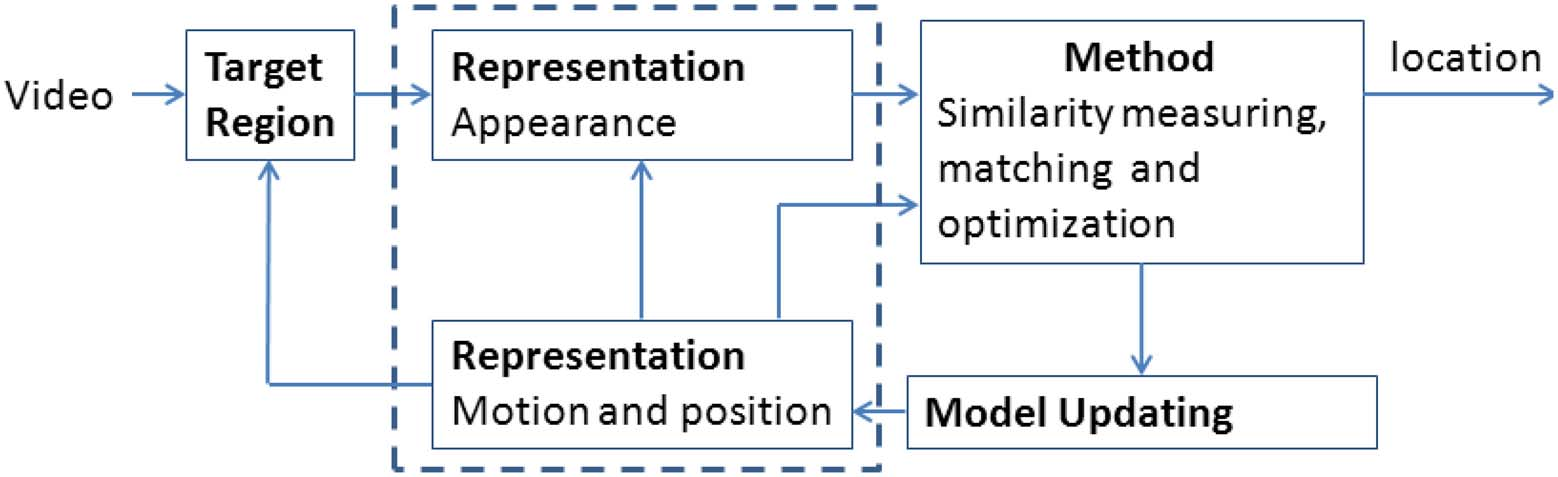
\includegraphics[width=12cm]{images/object_trackers_reference_model.png}
	\end{center}	
	\longcaptionsource{Ogólny model działania algorytmów śledzenia obiektów w sekwencjach video}{\textit{Target region} - Obszar zainteresowania (obszar obrazu zawierający obiekt zainteresowania)\\\textit{Representation - appearance} - Model  obiektu zainteresowania określający jego cechy charakterystyczne\\\textit{Representation - motion and position} - Model ruchu obiektu zainteresowania\\\textit{Method - similarity measuring, matching and optimization} - metoda pomiaru podobieństwa oraz stwierdzenia dopasowania obiektu pomiędzy klatkami\\\textit{Model updating} - metoda aktualizowania modelu cech obiektu zainteresowania	
}{\cite{Smeulders2010}}
\label{fig:Ogolny_model_dzialania_algorytmow_sledzenia_obiektow}
\end{figure}

\subsubsection{Reprezentacje obiektu na obrazie}
\label{subsubsec:Reprezentacje_obiektu_na_obrazie}

Pierwszym krokiem po uzyskaniu informacji o wystąpieniu obiektu jest zdefiniowanie jego reprezentacji rozumianej tutaj jako wyodrębnione składowe elementy obrazu przynależące do tego obiektu.

W najprostszym przypadku obiekt przybliża się jego \textbf{bryłą brzegową}, o postaci prostokąta lub elipsy zawierającej wszystkie należące do niego piksele. Inaczej mówiąc reprezentację obiektu stanowi fragment obrazu, który go zawiera. Zaletą takiego rozwiązania jest minimalna liczba parametrów opisująca obiekt, wadą natomiast włączeniem do jego reprezentacji dużej liczby pikseli tła \cite{Smeulders2010}.

Pewnym ulepszeniem tej koncepcji, zwiększającym jej odporność, jest stosowanie \textbf{wielu brył brzegowych} jednocześnie. Takie rozwiązanie cechuje się również większą elastycznością w dalszych krokach algorytmu, w których realizowane jest poszukiwane położenia w kolejnej klatce (uproszczone w przypadku pojedynczej bryły brzegowej do jednego punktu) \cite{Smeulders2010}.

Inną możliwą, lecz rzadko stosowaną w tej rodzinie algorytmów reprezentacją jest \textbf{kontur} obiektu zainteresowania. Cechuje się ona małą rygorystycznością w stosunku do zmiany ogólnego wyglądu obiektu, jednak jej użycie jest ograniczone do przypadków, w których stosowanie deskryptorów kształtu zapewnia wysoką dokładność \cite{Smeulders2010}.

Pozornie podobny sposób reprezentacji polega na określeniu \textbf{ciągłego obszaru obrazu} zawierającego piksele należące do obiektu zainteresowania. Należy zwrócić uwagę, że taka reprezentacja obiektu nie jest równoznaczna jego sylwetce (ang. \textit{silhouette}), rozumianej jako sumę zbiorów pikseli konturu obiektu oraz zbioru pikseli zawartych wewnątrz wyznaczonej przez niego bryły. Różnica ta jest wynikiem sposobu wyznaczania tych dwóch reprezentacji. Przedstawienie obiektu w postaci ciągłego obszaru obrazu pozwala na jego precyzyjne oddzielnie od innych obiektów. Wymaga natomiast dużej odporności od metody jego wyznaczenia, w celu uniknięcia wniesienia błędnej informacji o samym obiekcie \cite{Smeulders2010}.  

Nieco bardziej złożona reprezentacja obiektu oparta jest jest o \textbf{skrawki obrazu}. Są to małe obszary obrazu zawierające fragmenty obiektu zainteresowania, którego wygląd może zmieniać się niezależnie w ich obrębie. Odmianą tego modelu jest reprezentacja w postaci punktów charakterystycznych (ang. \textit{sailent points} lub \textit{interest points}), w których występuje pewna cecha charakterystyczna (ang. \textit{feature}) obrazu. Istnieją różne koncepcje definicji zbioru oraz relacji pomiędzy skrawkami obrazu \cite{Smeulders2010}. Cechą charakterystyczną takiej reprezentacji jest brak konieczności wyraźnego rozróżnienia pomiędzy tłem a obiektem zainteresowania. Skutkuje ona zwiększoną odpornością na przysłonięcia oraz zmianę kształtu obiektu zainteresowania. Z drugiej strony, w przypadku małych lub sztywnych obiektów reprezentacja skrawkami obrazu nie jest bardziej wydajna od reprezentacji opierających się o zbiory pojedynczych pikseli (jak np. w postaci bryły brzegowej) \cite{Smeulders2010}.

Na rysunku \ref{fig:Reprezentacje_obiektu_na_obrazie} przedstawiono przykładowy obiekt zainteresowania oraz wizualizacje odpowiadających mu reprezentacje według omówionych koncepcji.

\begin{figure}[!htb]
	\begin{center}
		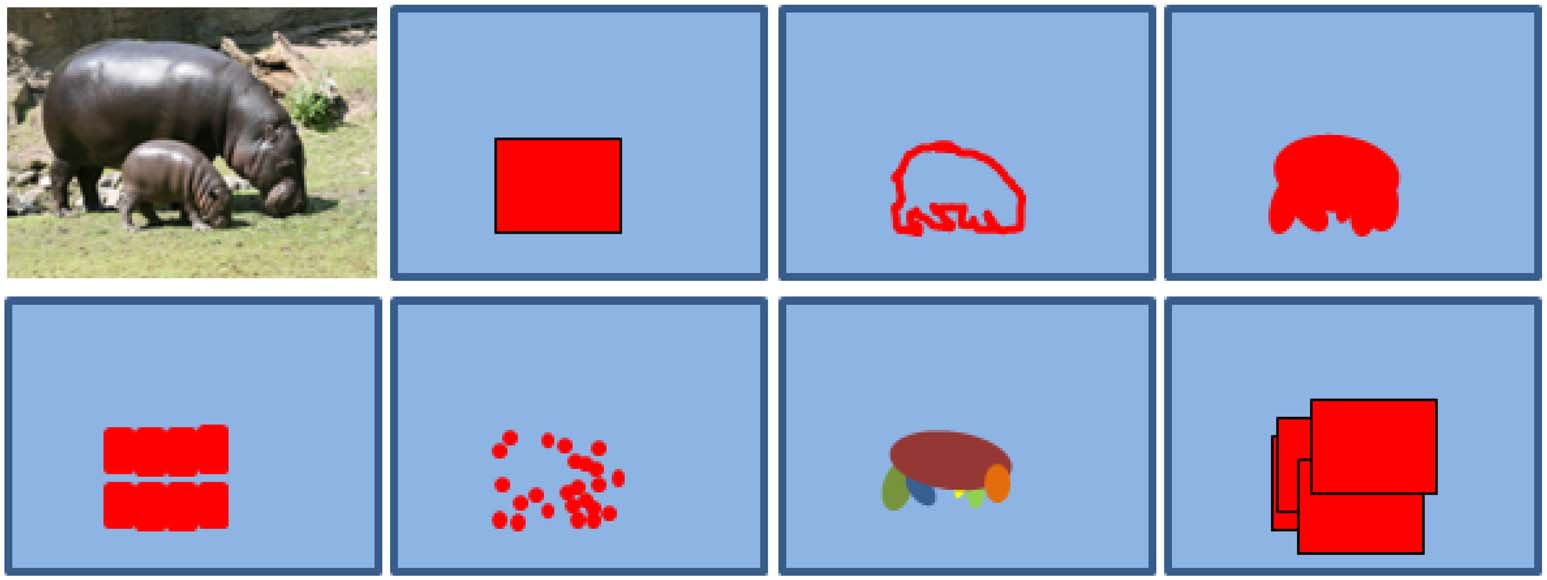
\includegraphics[width=12cm]{images/target_region_representation.png}
	\end{center}	
	\longcaptionsource{Reprezentacje obiektu zainteresowania na obrazie}{Kolejno, od lewego górnego rogu: obraz wejściowy, bryła brzegowa (ang. \textit{bounding box}), kontur obiektu, obszar obiektu (ang. \textit{blob}), skrawki obrazu (ang. \textit{image patches}), rozproszony zbiór punktów zainteresowania, części obiektu, wiele brył brzegowych}{\cite{Smeulders2010}}
\label{fig:Reprezentacje_obiektu_na_obrazie}
\end{figure}

\subsubsection{Modele obiektu zainteresowania}
\label{subsubsec:Modele_obiektu_zainteresowania}

Model obiektu, rozumiany jako opis jego cech charakterystycznych, tworzony jest w obrębie zdefiniowanego wcześniej obszaru zainteresowania (\ref{subsubsec:Reprezentacje_obiektu_na_obrazie}). Podstawowym wymaganiem, które musi spełniać jest zdolność do zachowania określonej właściwości pomiędzy kolejnymi klatkami, bez której wykonanie zadania śledzenia obiektu nie jest możliwe \cite{Smeulders2010}.

Istnieją trzy podstawowe reprezentacje cech charakterystycznych obiektu stosowane w algorytmach śledzenia: dwuwymiarowa tablica wartości pikseli, histogram oraz wektor cech \cite{Smeulders2010}.

Najbardziej oczywistą i bezpośrednią jest reprezentacja w postaci \textbf{dwuwymiarowej tablicy wartości pikseli obiektu} (rysunek \ref{fig:Modele_obiektu_zainteresowania}, punkt [a]). Najczęściej w tablicy przechowywane są wartości określające jasności poszczególnych pikseli \cite{Smeulders2010}, pomimo idącego za tym założenia dotyczącego jej stałych wartości, które rzadko jest prawdziwe. Tym niemniej taka reprezentacja nie powoduje utraty informacji o obiekcie wewnątrz obszaru zainteresowania.

Reprezentacja w postaci \textbf{histogramu} (rysunek \ref{fig:Modele_obiektu_zainteresowania}, punkt [b]) wyznaczana jest najczęściej w oparciu kolor pikseli w obszarze zainteresowania, występuje również w wersji przechowującej jedynie ich jasności \cite{Smeulders2010}. Przy reprezentacji w tej postaci następuje całkowita utrata informacji o właściwościach przestrzennych obiektu, przechowywana jest jedynie informacja o wartościach poszczególnych pikseli, co skutkuje największą elastycznością w odniesieniu do zmiany kształtu obiektu \cite{Smeulders2010}.

Reprezentacja w postaci \textbf{wektora cech} (rysunek \ref{fig:Modele_obiektu_zainteresowania}, punkt [c]) polega na wykryciu oraz deskrypcji cech charakterystycznych obiektu (ang. \textit{features}). W jej przypadku również nie przechowuje się informacji o kształcie geometrycznym obiektu \cite{Smeulders2010}. Cechy wraz z ich deskryptorami odwzorowują obiekt w oparciu o jego najbardziej bogate w informację właściwości, pozwalając na ograniczenie rozmiaru jego reprezentacji \cite{Smeulders2010}.

\begin{figure}[!htb]
	\begin{center}
		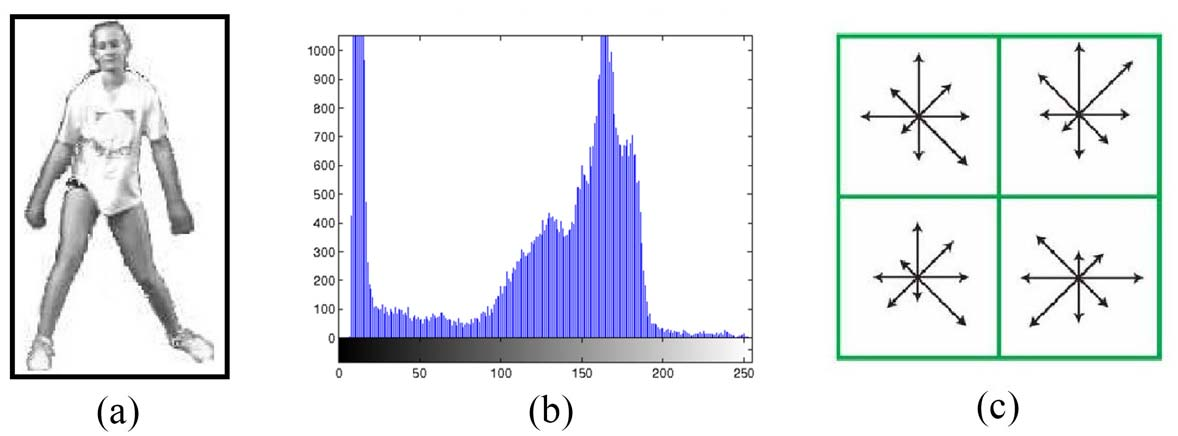
\includegraphics[width=12cm]{images/target_appearance_representation.png}
	\end{center}	
	\longcaptionsource{Modele obiektu zainteresowania, stosowane w algorytmach śledzenia obiektów}{a) Tablica dwuwymiarowa b) Histogram c) Wektor cech}{\cite{Smeulders2010}}
\label{fig:Modele_obiektu_zainteresowania}
\end{figure}

\subsubsection{Modele ruchu obiektu}
\label{subsubsec:Modele_ruchu_obiektu}

Przyjęcie założeń dotyczących ruchu obiektu (w tym sensie, stworzenie jego uproszczonego modelu) ma za zadanie zawężenie okna, w którym następuje próba stwierdzenia wystąpienia obiektu na kolejnej klatce sekwencji.

Najprostszy model nie narzuca żadnych ograniczeń poza założeniem, że obiekt po wykonaniu przemieszczenia pomiędzy kolejnymi klatkami znajduje się blisko pozycji początkowej \cite{Smeulders2010}. Jego implikacją jest stwierdzenie możliwości lokalizacji kolejnego położenia obiektu poprzez przeszukanie małego okna wokół poprzedniego \cite{Smeulders2010}, skąd nazwa \textbf{przeszukiwanie jednorodne}. Dzięki braku założeń dotyczących charakteru samego ruchu, rozwiązanie to cechuje duża ogólna odporność, nie sprawdza się ono jednak, jeśli ruch obiektu jest szybki \cite{Smeulders2010}.

Rozwinięciem koncepcji opisanej wyżej jest \textbf{gaussowski model ruchu}, w którym wprowadza prawdopodobieństwo wystąpienia kolejnego położenia obiektu wokół położenia początkowego zmienia się zgodnie z rozkładem normalnym. W tej reprezentacji dopasowaniu obiektu na kolejnej klatce przypisywany jest dodatkowo współczynnik wagowy (w oparciu o prawdopodobieństwo), co pozwala na zwiększenie przestrzeni poszukiwania \cite{Smeulders2010}.

Innym możliwym modelem jest \textbf{predykcja ruchu} obiektu z wykorzystaniem jego liniowego modelu oraz filtru Kalmana \cite{Smeulders2010}. Taką reprezentację można dodatkowo ulepszyć, wykonując predykcję w oparciu o przepływ optyczny \cite{Smeulders2010}.

W \textbf{bezpośredniej predykcji ruchu} nie przyjmuje się założeń odnośnie modelu ruchu, wykorzystuje się natomiast metody optymalizacji do znalezienia najlepiej dopasowanego nowego położenia w oparciu o położenia występujące wcześniej \cite{Smeulders2010}. Taki model jest jednak mało użyteczny, ponieważ wymaga, aby przemieszczenia obiektu były małe w porównaniu do innych zmian występujących na obrazie \cite{Smeulders2010}.

Ostatnia z metod reprezentacji polega na równoległym \textbf{śledzeniu i detekcji} obiektu z zastosowaniem niezależnych algorytmów. Po takim podejściu można oczekiwać dużej odporności na przypadkowe ruchu zarówno obiektu jak i kamery \cite{Smeulders2010}, jednak cechuje się ono największą komplikacją.

Na rysunku \ref{fig:Modele_ruchu_obiektu} zestawiono i porównano przedstawione wyżej sposoby modelowania ruchu. 

\begin{figure}[!htb]
	\begin{center}
		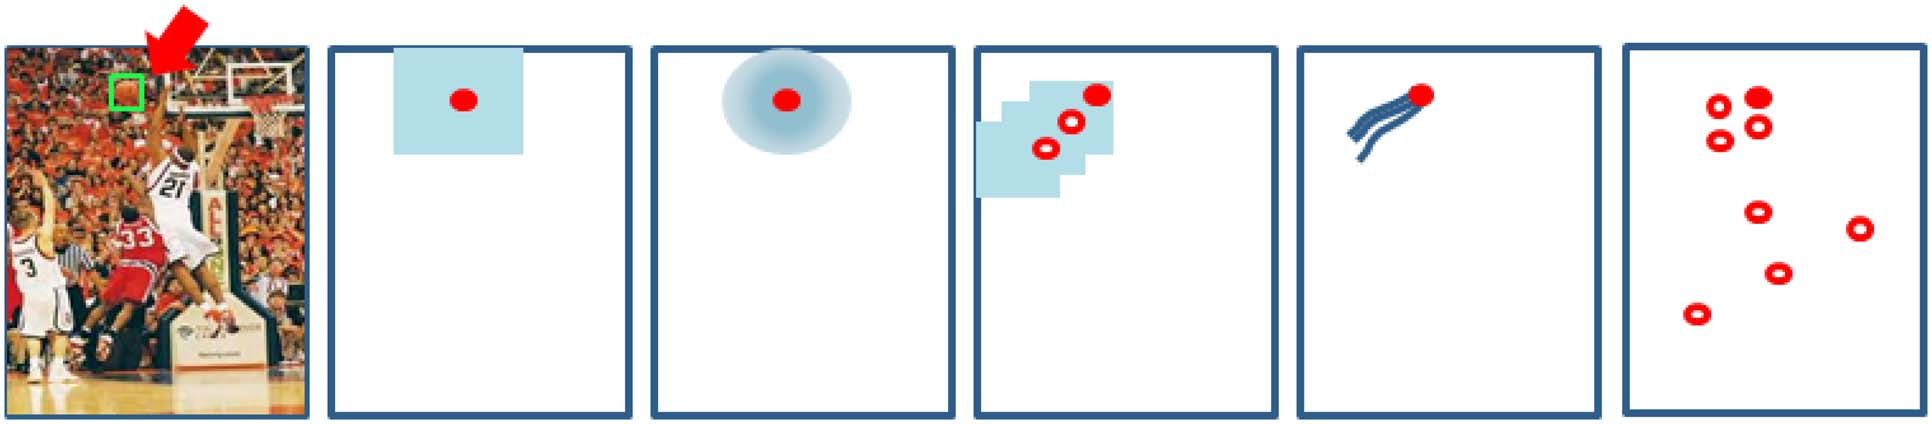
\includegraphics[width=12cm]{images/target_motion_representation.png}
	\end{center}	
	\longcaptionsource{Modele ruchu obiektu, stosowane w algorytmach śledzenia obiektów}{Od lewej: obiekt zainteresowania, przeszukiwanie jednorodne, gaussowski model ruchu, predykcja ruchu, model wprost, śledzenie i wykrywanie}{\cite{Smeulders2010}}
\label{fig:Modele_ruchu_obiektu}
\end{figure}

\subsubsection{Metody pomiaru podobieństwa oraz stwierdzenia dopasowania obiektu pomiędzy klatkami}
\label{subsubsec:Metody_pomiaru_podobienstwa_oraz_stwierdzenia_dopasowania_obiektu pomiedzy_klatkami}

Metoda pomiaru podobieństwa obiektu oraz stwierdzenia jego dopasowania pomiędzy klatkami to kluczowy element algorytmu śledzenia, które w tym właśnie etapie jest zasadniczo realizowane.

Pierwsza i najprostsza jej realizacja opiera się na wykonaniu \textbf{dopasowania} pomiędzy znanym modelem obiektu zainteresowania na początkowej klatce, do kandydatów, których modele tworzone są dla jego możliwych położeń na kolejnej klatce, zgodnie z przyjętym modelem ruchu. Jednemu znanemu obiektowi zainteresowania jest więc przypisywany zbiór jego możliwych kolejnych instancji (rysunek \ref{fig:Metody_sledzenia_obiektow_na_obrazach}, punkt [a]), spośród których wybierana jest najlepiej dopasowana.
Inaczej mówiąc, śledzenie w tym przypadku jest zdaniem optymalizacji. Na podstawie podejścia do jego rozwiązania można wyróżnić dwie kategorie - dopasowanie bezpośrednie, polegające na poszukiwaniu najlepszego kandydata wzdłuż gradientu pewnej funkcji określającej dopasowanie, oraz dopasowanie probabilistyczne, polegające na znalezieniu maksimum funkcji gęstości prawdopodobieństwa, opisującej prawdopodobieństwo wystąpienia obiekt zainteresowania w danych punkcie obrazu. Dopasowanie bezpośrednie wykazuje dużą odporność przy wielu różnych modelach ruchu obiektu, przy zachowaniu warunku małej przestrzeni przeszukiwania. Z drugiej strony opiera się one o silne założenia dotyczące opisu modelu obiektu, w skutek jest wrażliwe na lokalne zmiany intensywności pikseli (występujące w rzeczywistych sekwencjach obrazów, w wyniku np. zmiany kąta padania światła) oraz jakość reprezentacji obiektu na obrazie \cite{Smeulders2010}. Dopasowanie probabilistyczne jest efektywne w przypadku możliwości wystąpienia przysłonięcia obiektu oraz niejednoznaczności, pojawiających się np. przy wielu podobnych obiektach \cite{Smeulders2010}.

\textbf{Dopasowanie z rozszerzonym opisem cech} rozszerza koncepcję dopasowania o opis modelu lub stan metody w przeszłości (dla ciągu przednich klatek) \cite{Smeulders2010}. Przy takim podejściu wieloelementowemu zbiorowi znanych wystąpień obiektu zainteresowania w ciągu poprzednich klatek przyporządkowywany jest wieloelementowy zbiorów kandydatów nowej instancji tego obiektu na klatce bieżącej (rysunek \ref{fig:Metody_sledzenia_obiektow_na_obrazach}, punkt [b]). Metoda przechowuje długotrwale trajektorię stanu obiektu zainteresowania, w związku z czym jest użyteczne w zadaniach śledzenia długoterminowego oraz w przypadku możliwości wystąpienia przysłonięć \cite{Smeulders2010}. Dopasowywanie jest wykonywane pomiędzy poszczególnymi elementami obydwu zbiorów, co skutkuje zwiększeniem złożoności obliczeniowej. 

W celu jej ograniczenia wprowadzono \textbf{dopasowywanie z więzami}, przy którym podobieństwo pomiędzy zbiorami wystąpień i kandydatów jest rozpatrywane jedynie dla elementów spełniających zdefiniowane kryteria, lub inaczej, więzy (rysunek \ref{fig:Metody_sledzenia_obiektow_na_obrazach}, punkt [c]). Mogą dotyczyć one, np. zmiany koloru lub kształtu obiektu pomiędzy kolejnymi klatkami. Metody tego typu mogą dobrze sprawdzać się w warunkach dużej zmienności obserwowanej sceny, nadają się również do zastosowania w algorytmach śledzących predefiniowanych wzorców \cite{Smeulders2010}.

Alternatywą dla metod opierających się o dopasowanie jest \textbf{klasyfikacja rozróżniająca}, określana inaczej jako ,,śledzenie przez wykrywanie'' \cite{Smeulders2010}. Opiera się ona o założenie, że samo odróżnienie pojedynczego obiektu zainteresowania od tła jest wystarczające do jego śledzenia \cite{Smeulders2010}. Klasyfikacja rozróżniająca polega więc na określeniu przynależności wszystkich pikseli obrazu do tła bądź obiektu zainteresowania, oraz uaktualnianiu informacji o tej przynależności na kolejnych klatkach sekwencji video. W tej metodzie występuje więc przyporządkowanie pomiędzy oznaczonym obiektem zainteresowania i jego tłem poprzedniej klatce oraz zbiorem par kandydat-tło na kolejnej (rysunek \ref{fig:Metody_sledzenia_obiektow_na_obrazach}, punkt [d]). Klasyfikator może przetwarzać zestaw wielu różnych cech jednocześnie, co pozwala na osiągnięcie dużej odporności w przypadku niskiej specjalizacji algorytmu śledzącego oraz wysokiej niestabilności obserwowanej sceny \cite{Smeulders2010}. U podstaw metody leży jednak domniemanie unikalności cech śledzonego obiektu w skali obrazu, co powoduje jej błędne działanie w przypadku jego wielokrotnego wystąpienia \cite{Smeulders2010}. Jest ona także wrażliwa na błędne etykietowanie pikseli, prowadzące do zakłócenia pracy klasyfikatora oraz przekłamania śledzonej trajektorii obiektu zainteresowania (ang. \textit{drift}).  

\textbf{Klasyfikacja rozróżniająca z więzami} jest rozwinięciem poprzedniej rodziny metod, wśród których główny nacisk kładzie się na poprawną klasyfikację i etykietowanie pikseli, a nie na poszukiwanie najlepszej (najbardziej dopasowanej lub prawdopodobnej) pozycji śledzonego obiektu \cite{Smeulders2010}. Polega ono na syntezie informacji o przynależności zbioru pikseli do obiektu z poszukiwaniem w jego otoczeniu obszaru najlepiej dopasowanego do stworzonego uprzednio modelu, w postaci np. wektora cech (rysunek \ref{fig:Metody_sledzenia_obiektow_na_obrazach}, punkt [e]). Wadą tej metody jest wysoka złożoność obliczeniowa, wynikająca ze stopnia jej komplikacji.

\begin{figure}[!htb]
	\begin{center}
		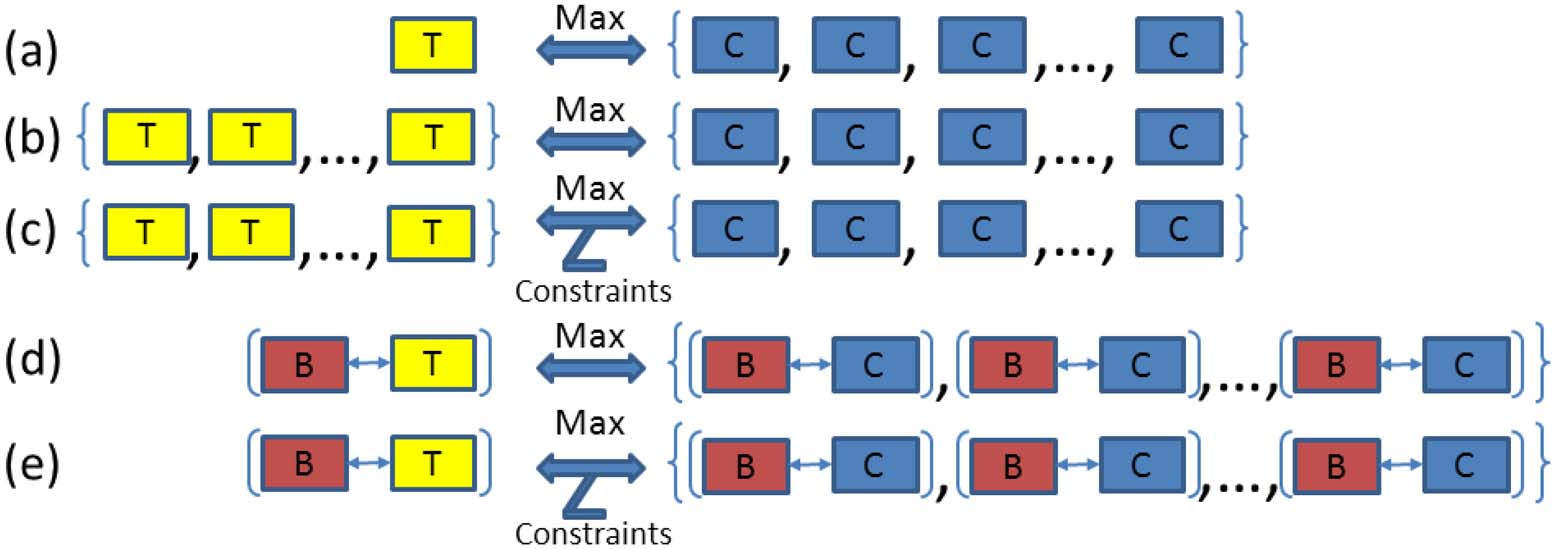
\includegraphics[width=12cm]{images/target_tracking_methods.png}
	\end{center}	
	\longcaptionsource{Metody śledzenia obiektów na obrazach}{a) Dopasowanie b) Dopasowanie z rozszerzonym opisem cech c) Dopasowanie z więzami d) Klasyfikacja rozróżniająca e) Klasyfikacja rozróżniająca z więzami. Oznaczenia bloków: T - wystąpienie obiektu zainteresowania, C - potencjalne kolejne wystąpienie obiektu zainteresowania, B - lokalne wystąpienia tła.}{\cite{Smeulders2010}}
\label{fig:Metody_sledzenia_obiektow_na_obrazach}
\end{figure}

\subsubsection{Metody uaktualnienia modelu obiektu zainteresowania}
\label{subsubsec:Metody_uaktualnienia_modelu_obiektu_zainteresowania}

Ostatni krok algorytmu śledzenia obiektu polega na uaktualnieniu stosowanego modelu na podstawie informacji zawartych w nowej klatce sekwencji video. W niektórych przypadkach nie jest on konieczny - poza uproszczeniem całego algorytmu, zaletą takiego rozwiązania jest brak wnoszenia błędnej informacji o obiekcie, która może być skutkiem niedoskonałego modelu \cite{Smeulders2010}.

Najprostsza realizacja uaktualnienia polega na \textbf{zastąpieniu} dotychczasowego opisu modelu opisem wykonanym dla ostatnio zaobserwowanego wystąpienia obiektu. Może się to odbywać w sposób częściowy, poprzez zastępowanie kolejnych fragmentów opisu nowymi, bądź przez okresowe, całościowe jego zastąpienie \cite{Smeulders2010}. 

\textbf{Predykcja} postaci modelu przy użyciu filtru Kalmana (\ref{subsub:Filtr_Kalmana}) jest koncepcyjnie podobna, pozwalając jednocześnie na ograniczenie wpływu zakłóceń, zwłaszcza jeśli przebieg trajektorii obiektu jest łagodny. Gwałtowne jej zmiany skutkują jednak wniesieniem dodatkowego błędu \cite{Smeulders2010}. 

W przypadku reprezentacji obiektu w postaci skrawków obrazu, uaktualnianie modelu polega na odpowiednim ich wstawianiu, usuwaniu, zmienieniu i przesuwaniu. Jest to zadanie złożone, dodatkowo rozwiązywane w oparciu o ograniczony zasób informacji \cite{Smeulders2010}.

Dla algorytmów wykorzystujących rozszerzony opis cech obiektów stosowana jest przyrostowa analiza głównych składowych \cite{Smeulders2010}. Pozwala ona na przechowanie informacji o stanie modelu w przeszłości. 

\subsection{Algorytmy śledzenia obiektów na obrazach w robotyce mobilnej}
\label{subsec:Algorytmy_sledzenia_obiektow_na_obrazach_w_robotyce_mobilnej}

\subsubsection{Śledzenie z wykorzystaniem przepływu optycznego}
\label{subsubsec:Sledzenie_z_wykorzystaniem_przeplywu_optycznego}

Jak wspomniano wspomniano w podrozdziale \ref{subsec:Analiza_ruchu_i_przeplyw_optyczny} przepływ optyczny jest użytecznym narzędziem w analizie ruchu obiektów zarejestrowanego w sekwencji obrazów. 

\subsubsection{Śledzenie z wykorzystaniem cech obiektu}
\label{subsubsec:Sledzenie_z_wykorzystaniem_cech}